\documentclass[11pt]{article}
\usepackage[margin=1in]{geometry}
\usepackage{booktabs}
\usepackage{graphicx}
\usepackage{float}
\usepackage{hyperref}
\usepackage{enumitem}
\hypersetup{colorlinks=true, linkcolor=blue, urlcolor=blue}
\setlength{\parindent}{0pt}
\setlength{\parskip}{0.6em}

\title{Where Degenerate Rollouts Enter: OLMo and Qwen Combined Read}
\author{}
\date{2026-04-09 01:40 UTC}

\begin{document}
\maketitle

\section*{Executive Summary}
\begin{itemize}[leftmargin=1.5em]
\item The corrected OLMo3 audit still does not support ``RLVR introduces the degeneration.'' The repaired bounded rows moved the old fishy OLMo3 failures back onto a coherent surface.
\item The scaled OLMo2 \texttt{1B} ladder remains the cleanest stage progression object on this thread: heavy loop / max-length-hit mass is already present in base, drops sharply in SFT, is usually smallest at \texttt{RLVR1}, and can re-accumulate in final instruct on some harder datasets.
\item The Qwen same-family control is now finished too. Under the old Qwen3 rollout-stat sampler, \texttt{Qwen/Qwen3-1.7B-Base} with raw prompting showed substantial loop and max-length-hit mass on all five datasets, not just the earlier \texttt{MATH-500} anchor row.
\item So the base/raw pathology is not OLMo-only. What changes across families is the failure mode:
\begin{itemize}[leftmargin=1.5em]
\item OLMo2 base repeats derivation content or falls into synthetic-junk tails.
\item Qwen base raw often loops on the answer-format instruction tail on MCQ, while still showing a smaller real math loop regime under the long-horizon control.
\end{itemize}
\end{itemize}

\section*{Objects and Caveats}
\textbf{OLMo3 corrected audit.}
The repaired bounded OLMo3 rows that replaced the fishy ones are:
\begin{itemize}[leftmargin=1.5em]
\item \texttt{SFT / MMLU-Pro = 34 / 80} correct, \texttt{1 / 80} looped, \texttt{1 / 80} max-hit
\item \texttt{RLVR / MMLU-Pro = 27 / 80} correct, \texttt{0 / 80} looped, \texttt{0 / 80} max-hit
\item \texttt{SFT / LiveCodeBench = 6 / 80} correct, \texttt{1 / 80} looped, \texttt{1 / 80} max-hit
\item \texttt{RLVR / LiveCodeBench = 22 / 80} correct, \texttt{0 / 80} looped, \texttt{0 / 80} max-hit
\end{itemize}
The only clean OLMo3 base-versus-instruct comparison still on disk is the corrected \texttt{32}-prompt \texttt{MATH-500} pilot:
\begin{itemize}[leftmargin=1.5em]
\item base \texttt{raw}: \texttt{9 / 32} correct, \texttt{3 / 32} looped, \texttt{0 / 32} max-hit
\item SFT \texttt{chat\_template}: \texttt{17 / 32} correct, \texttt{0 / 32} looped, \texttt{0 / 32} max-hit
\item RLVR \texttt{chat\_template}: \texttt{16 / 32} correct, \texttt{0 / 32} looped, \texttt{0 / 32} max-hit
\end{itemize}

\textbf{OLMo2 \texttt{1B} ladder.}
This is the scaled stage object:
\begin{itemize}[leftmargin=1.5em]
\item \texttt{temperature=0.1}, \texttt{top\_p=0.95}, \texttt{top\_k=-1}, \texttt{num\_generations=10}
\item \texttt{max\_tokens=max\_model\_len=4096}
\item \texttt{50} prompts per dataset
\item stages: base \texttt{->} SFT \texttt{->} \texttt{RLVR1} \texttt{->} instruct
\end{itemize}

\textbf{Qwen same-family base control.}
The new base run replays the old sampler on \texttt{Qwen/Qwen3-1.7B-Base}:
\begin{itemize}[leftmargin=1.5em]
\item \texttt{temperature=0.2}, \texttt{top\_p=0.95}, \texttt{top\_k=-1}, \texttt{num\_generations=10}, \texttt{max\_tokens=81920}
\item real base context limit \texttt{max\_model\_len=32768}, not the instruct checkpoint's \texttt{40960}
\item math / MCQ datasets on explicit \texttt{raw}
\item \texttt{LiveCodeBench release\_v6} on raw benchmark strings with \texttt{LM\_STYLE=GenericBase}
\end{itemize}
Important caveat: the saved instruct-side \texttt{LiveCodeBench} reference used \texttt{LM\_STYLE=CodeQwenInstruct}, and the base bundle is bounded to \texttt{50} prompts per dataset while the saved instruct reference uses the older larger dataset caps. So treat this as a same-family control, not a literal same-surface stage ladder.

\section*{OLMo Read}
\begin{figure}[H]
\centering
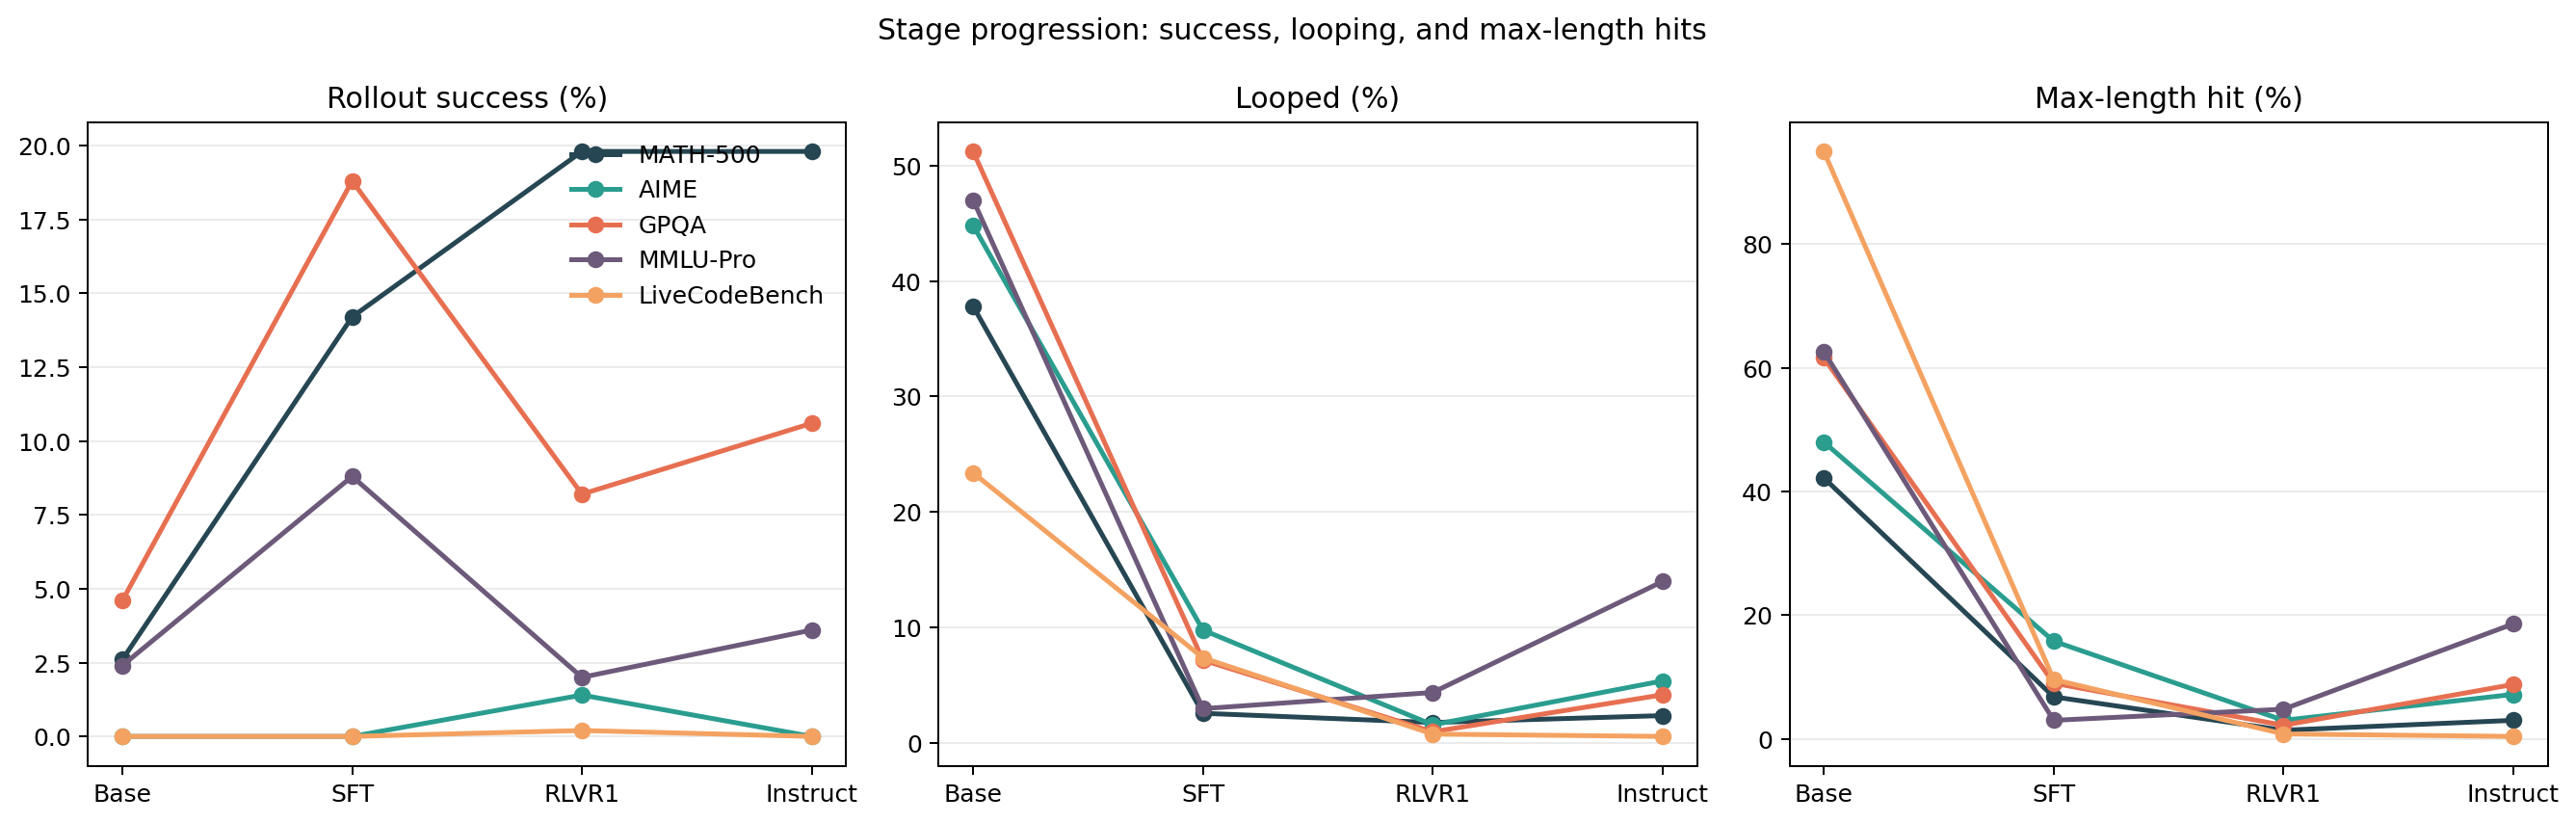
\includegraphics[width=\textwidth]{figures/olmo2_progression_rates.png}
\caption{Scaled OLMo2 \texttt{1B} stage progression. This is the cleanest available full-ladder object for the question ``where does the degenerate-rollout regime enter the family?''}
\end{figure}

\begin{figure}[H]
\centering
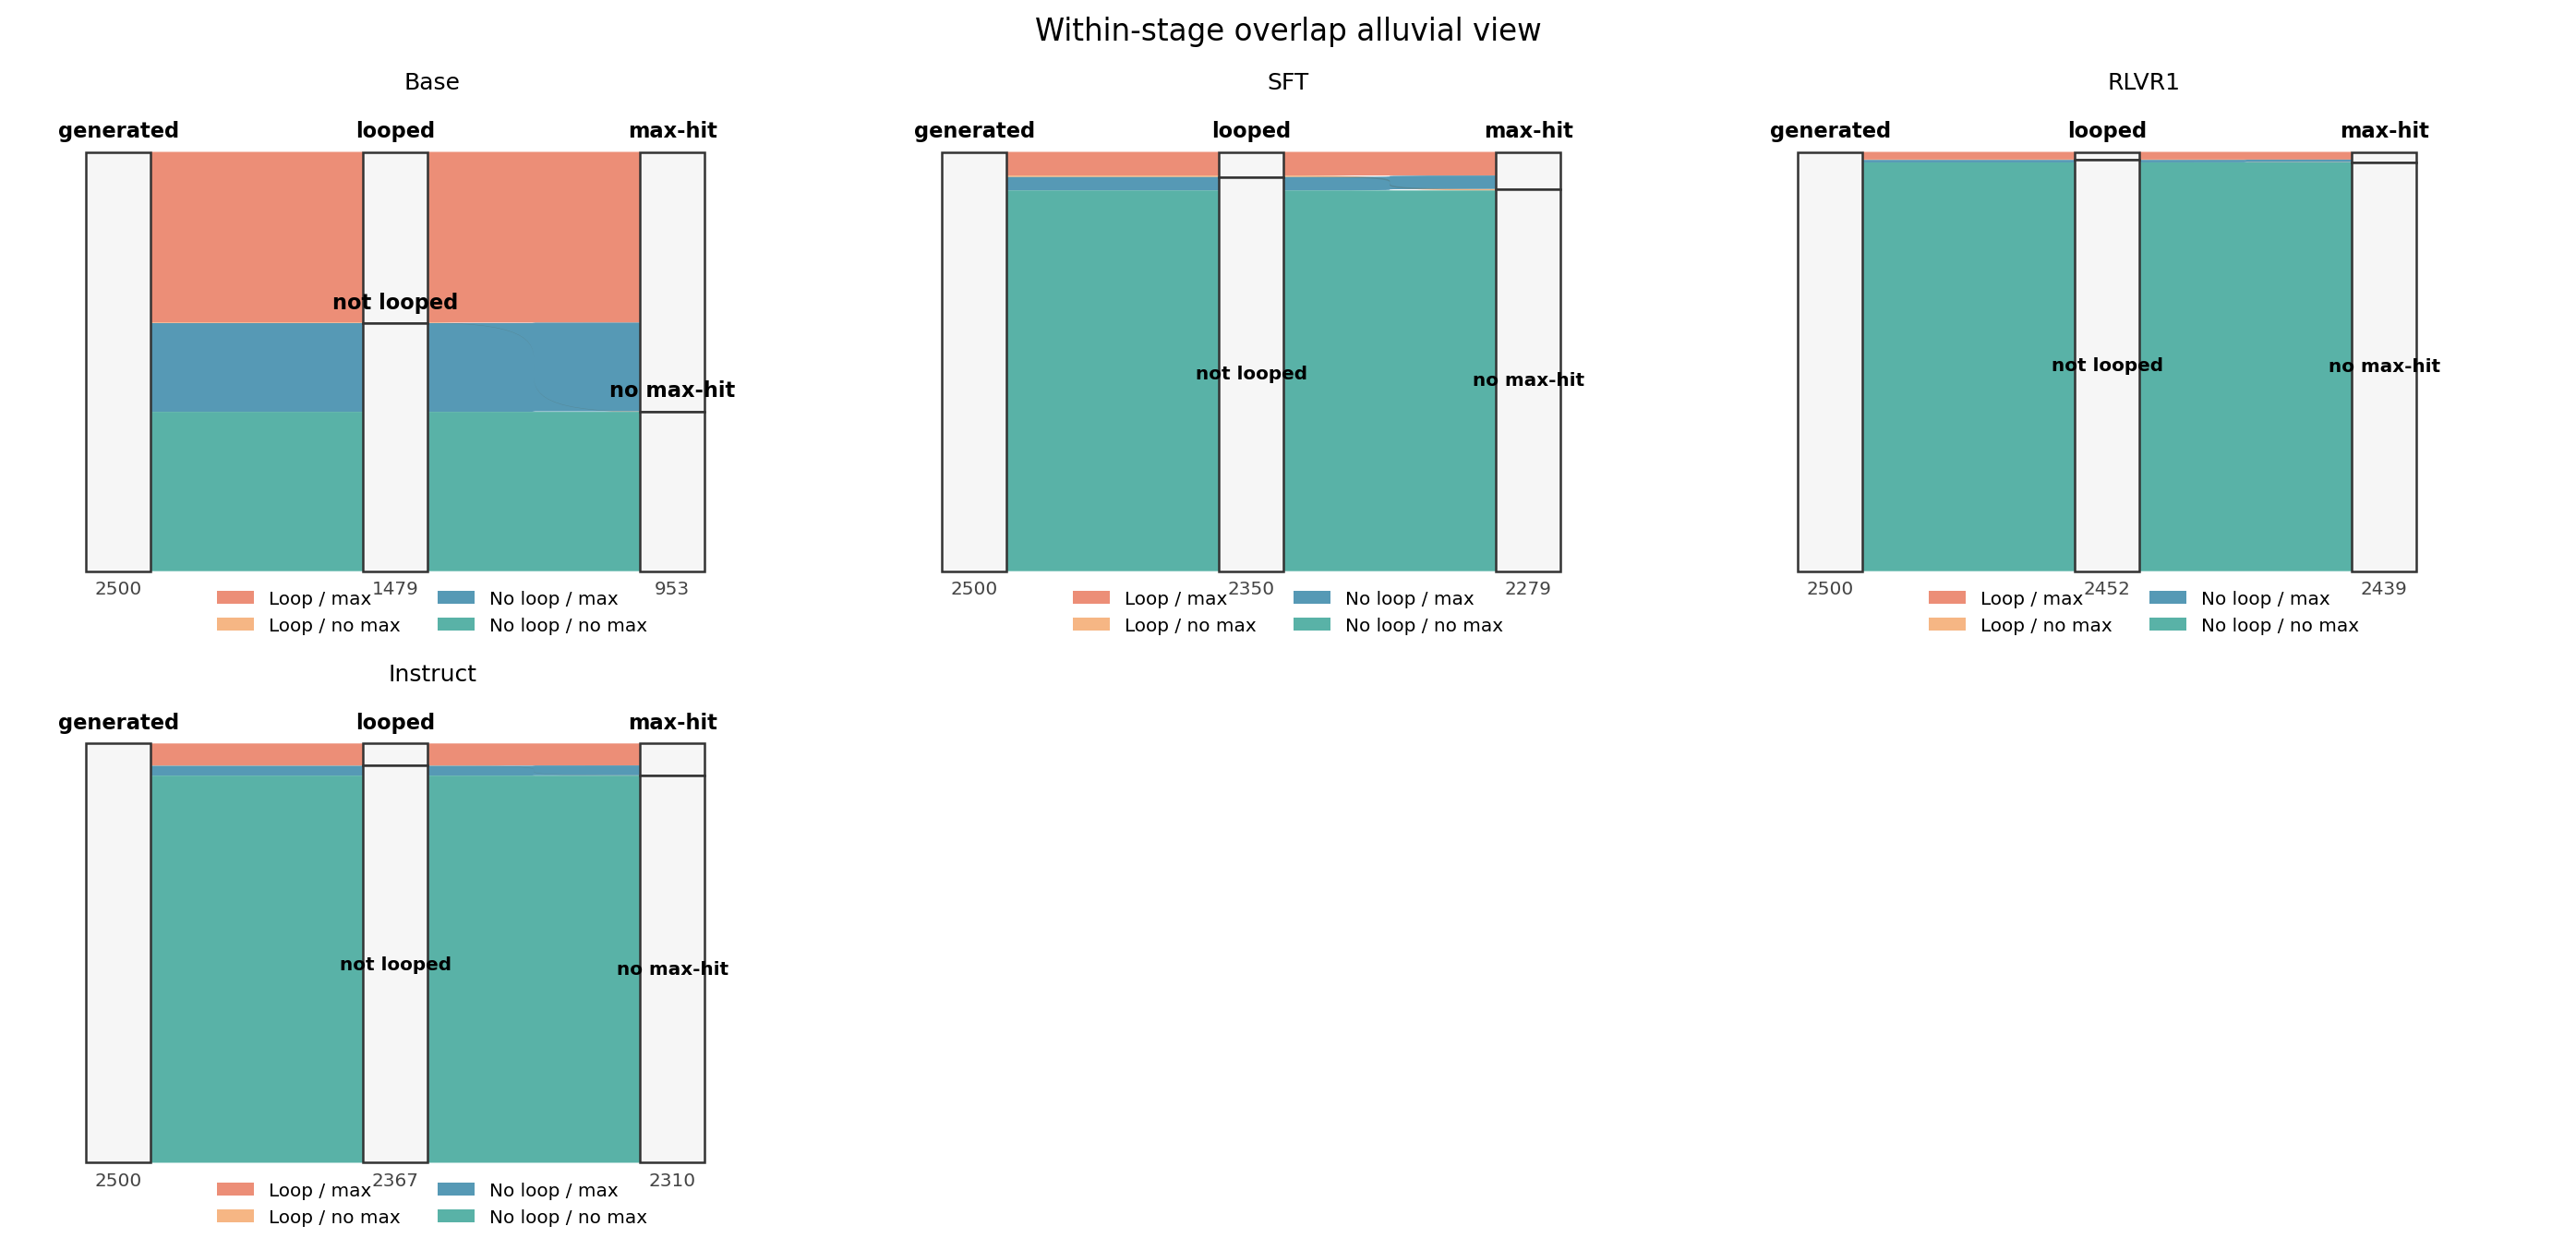
\includegraphics[width=\textwidth]{figures/olmo2_stage_overlap_sankey.png}
\caption{Within-stage overlap structure for the same OLMo2 \texttt{1B} ladder.}
\end{figure}

Anchor OLMo2 rows from the \texttt{50}-prompt ladder:
\begin{itemize}[leftmargin=1.5em]
\item base:
\begin{itemize}[leftmargin=1.5em]
\item \texttt{MATH-500}: \texttt{189 / 500} looped, \texttt{211 / 500} max-hit
\item \texttt{AIME}: \texttt{224 / 500} looped, \texttt{240 / 500} max-hit
\item \texttt{GPQA}: \texttt{256 / 500} looped, \texttt{308 / 500} max-hit
\item \texttt{MMLU-Pro}: \texttt{235 / 500} looped, \texttt{313 / 500} max-hit
\item \texttt{LiveCodeBench}: \texttt{117 / 500} looped, \texttt{475 / 500} max-hit
\end{itemize}
\item \texttt{RLVR1}:
\begin{itemize}[leftmargin=1.5em]
\item \texttt{MATH-500}: \texttt{9 / 500} looped, \texttt{7 / 500} max-hit
\item \texttt{AIME}: \texttt{8 / 500} looped, \texttt{15 / 500} max-hit
\item \texttt{GPQA}: \texttt{5 / 500} looped, \texttt{11 / 500} max-hit
\item \texttt{MMLU-Pro}: \texttt{22 / 500} looped, \texttt{24 / 500} max-hit
\item \texttt{LiveCodeBench}: \texttt{4 / 500} looped, \texttt{4 / 500} max-hit
\end{itemize}
\item final instruct remains mixed rather than monotone:
\begin{itemize}[leftmargin=1.5em]
\item \texttt{MMLU-Pro}: \texttt{70 / 500} looped, \texttt{93 / 500} max-hit, clearly worse than \texttt{RLVR1}
\end{itemize}
\end{itemize}

\section*{Qwen Read}
\begin{center}
\small
\setlength{\tabcolsep}{5pt}
\resizebox{\textwidth}{!}{
\begin{tabular}{@{}lrrrrrr@{}}
\toprule
Dataset & Base succ. & Base loop & Base max-hit & Instruct succ. & Instruct loop & Instruct max-hit \\
\midrule
\texttt{MATH-500} & 48.6\% & 3.8\% & 4.4\% & 72.6\% & 2.94\% & 1.46\% \\
\texttt{AIME} & 4.6\% & 22.8\% & 23.2\% & 38.5\% & 15.0\% & 12.7\% \\
\texttt{GPQA} & 8.2\% & 38.0\% & 38.0\% & 34.5\% & 16.4\% & 6.92\% \\
\texttt{MMLU-Pro} & 11.0\% & 31.4\% & 31.4\% & 65.2\% & 4.56\% & 0.95\% \\
\texttt{LiveCodeBench} & 20.4\% & 46.4\% & 46.8\% & 58.1\% & 15.0\% & 10.8\% \\
\bottomrule
\end{tabular}
}
\end{center}

\begin{figure}[H]
\centering
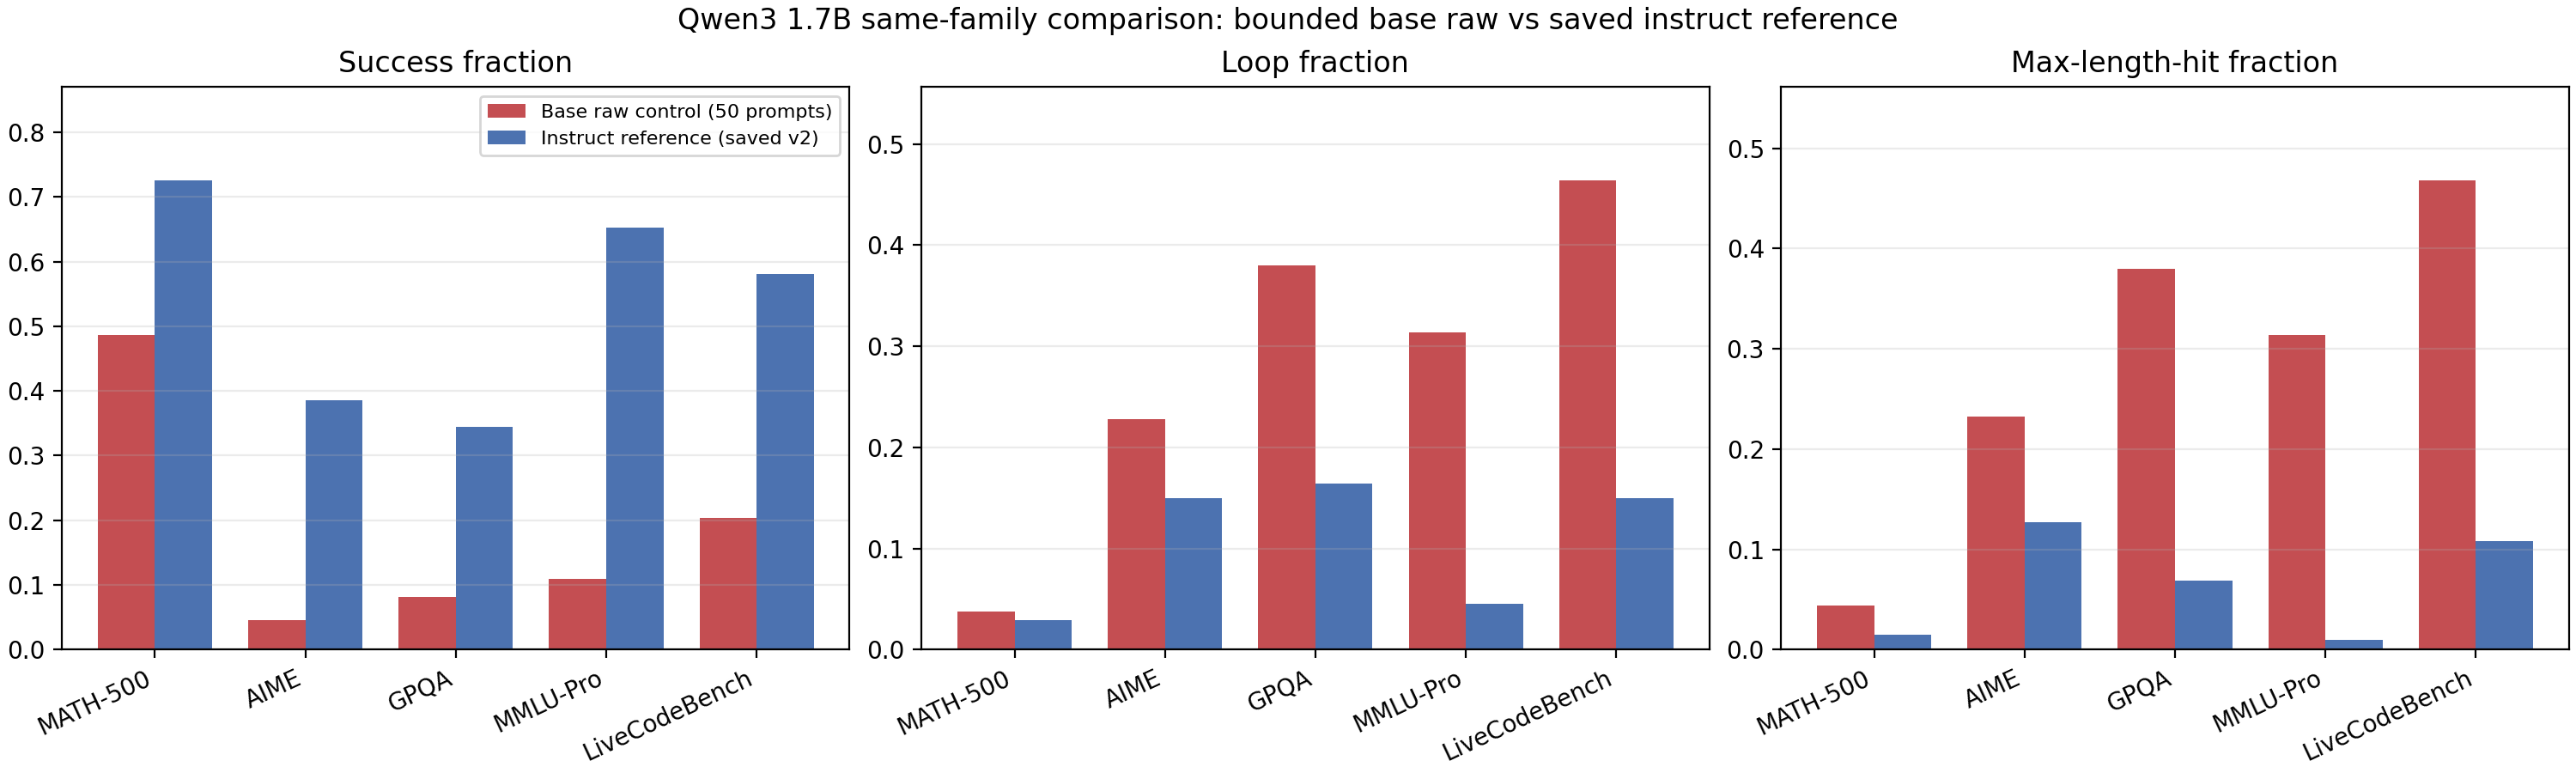
\includegraphics[width=\textwidth]{figures/qwen_base_vs_instruct_rates.png}
\caption{Bounded Qwen base/raw control versus the saved Qwen3 instruct reference. The comparison is same-family and sampler-aligned, but not perfectly same-surface: raw/chat and context-limit differences remain explicit.}
\end{figure}

\begin{figure}[H]
\centering
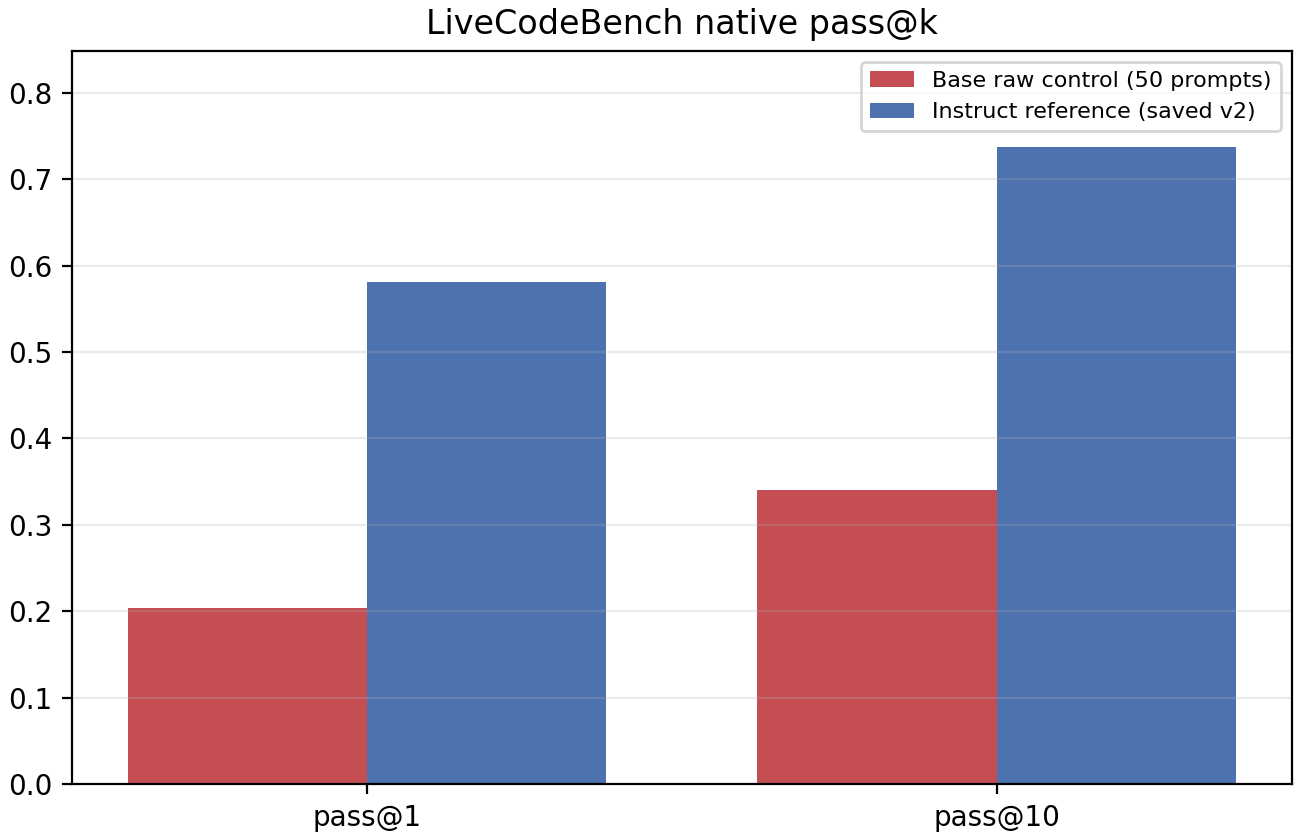
\includegraphics[width=0.65\textwidth]{figures/qwen_base_vs_instruct_lcb_passk.png}
\caption{Native \texttt{LiveCodeBench} \texttt{pass@k}. The base/raw control is weak but not a zero-capability surface: \texttt{pass@1 = 0.204}, \texttt{pass@10 = 0.34}.}
\end{figure}

Exact Qwen base/raw rows:
\begin{itemize}[leftmargin=1.5em]
\item \texttt{MATH-500}: \texttt{243 / 500} correct, \texttt{19 / 500} looped, \texttt{22 / 500} max-hit, mean length \texttt{1893.6}
\item \texttt{AIME}: \texttt{23 / 500} correct, \texttt{114 / 500} looped, \texttt{116 / 500} max-hit, mean length \texttt{8452.6}
\item \texttt{GPQA}: \texttt{41 / 500} correct, \texttt{190 / 500} looped, \texttt{190 / 500} max-hit, mean length \texttt{12498.8}
\item \texttt{MMLU-Pro}: \texttt{55 / 500} correct, \texttt{157 / 500} looped, \texttt{157 / 500} max-hit, mean length \texttt{10268.5}
\item \texttt{LiveCodeBench}: \texttt{102 / 500} rollout-correct, \texttt{232 / 500} looped, \texttt{234 / 500} max-hit, mean length \texttt{14858.8}, native \texttt{pass@1 = 0.204}, \texttt{pass@10 = 0.34}
\end{itemize}

Two extra points matter for interpretation:
\begin{itemize}[leftmargin=1.5em]
\item The \texttt{LiveCodeBench} wrapper caveat is real but not enough by itself to explain the result. On the tiny \texttt{2}-prompt style probe, both \texttt{GenericBase} and \texttt{CodeQwenInstruct} looped to the cap with \texttt{pass@1 = 0}.
\item Qwen's failure text still differs from OLMo2. The long MCQ failures often repeat the answer-format instruction tail itself (\texttt{Do not output anything else}, \texttt{Do not explain your answer}, \texttt{Do not output anything that is not JSON}), rather than repeating the math derivation content.
\end{itemize}

\section*{Bottom Line}
\begin{itemize}[leftmargin=1.5em]
\item The clean stage conclusion still comes from OLMo2 \texttt{1B}: heavy degeneracy is already present in base, then usually shrinks through SFT and RLVR rather than appearing from near zero.
\item The finished Qwen same-family control now shows that the base/raw degeneration object is not OLMo-only.
\item What changes across families is the failure mode, not the existence of the pathology.
\item The strongest caveat that remains is surface purity, not missing data:
\begin{itemize}[leftmargin=1.5em]
\item OLMo3 still lacks a finished full \texttt{7B} base five-dataset bundle.
\item Qwen base versus instruct is a same-family control, not a literal same-surface stage ladder, because wrapper, context limit, and dataset cap are not perfectly matched.
\end{itemize}
\end{itemize}

\end{document}
